\documentclass{report}

\usepackage[latin1]{inputenc}
\usepackage[english]{babel}
\usepackage{lmodern} %font
%\usepackage{url} % for clickable links
\usepackage[hidelinks]{hyperref} % for links in tableofcontent
\usepackage[top=3cm, bottom=4cm, left=4cm, right=4cm]{geometry} % for margins.
\usepackage[pdftex]{graphicx} % for images includes
\usepackage{titlesec}	% Remove the label ``chapter #''
\titleformat{\chapter}% But still display it in the ToC
  {\Large\bfseries} % format
  {}                % label
  {0pt}             % sep
  {\huge}           % before-code

\begin{document}

% the fancy title
\begin{titlepage}
\newcommand{\HRule}{\rule{\linewidth}{0.5mm}} % new command for the horizontal lines, change thickness here

\center % Center everything on the page
\textsc{\LARGE Halmstad's university}\\[1.5cm] % Name of your university/college
\textsc{\Large Advanced Oriented Object Programming}\\[0.5cm] % Major heading such as course name
%\textsc{\large Minor Heading}\\[0.5cm] % Minor heading such as course title
% title
\HRule \\[0.4cm]
{ \huge \bfseries Sound editor framework}\\[0.4cm] % Title of your document
\HRule \\[1.5cm]

% Authors
\begin{minipage}{0.4\textwidth}
\begin{flushleft} \large
\emph{Authors:}\\
R�mi \textsc{Gourdon}\\
Hichame \textsc{Moriceau} % Your name
\end{flushleft}
\end{minipage}
~
\begin{minipage}{0.4\textwidth}
\begin{flushright} \large
\emph{Supervisor:} \\
Dr. Veronica \textsc{Gaspes} % Supervisor's Name
\end{flushright}
\end{minipage}\\[4cm]
{\large \today}\\[3cm] % Date
\vfill % fill the rest of the page with whitespace
\end{titlepage}
% end of : fancy title


\tableofcontents % add summary


\chapter{Introduction}

Our framework offers to: synthesise, visualize and tweak sounds through different modifiers.
It comes with built-in generators, views, filters and effects, but, according to the project specifications, we did our best to make room for extensions.
Two implementations are provided, to demonstrate various ways of using it, and different manners of assembling its components.

The question of modularity was for us a top priority from day one. Indeed, audio creation is typically a domain where the possibilities are endless.
The sound generators can range from basic signal generators to complex synthesizer, either mimicking real instruments or creating completely new sounds.
The same goes for filters and effects, which can be as simple as low-pass and high-pass, delays, but also flangers, reverbs, etc.
For these modules, that we called modifiers, we also quickly realized that the possibility of adding several of them to the same sound would really expand the possibilities.

\chapter{Design}

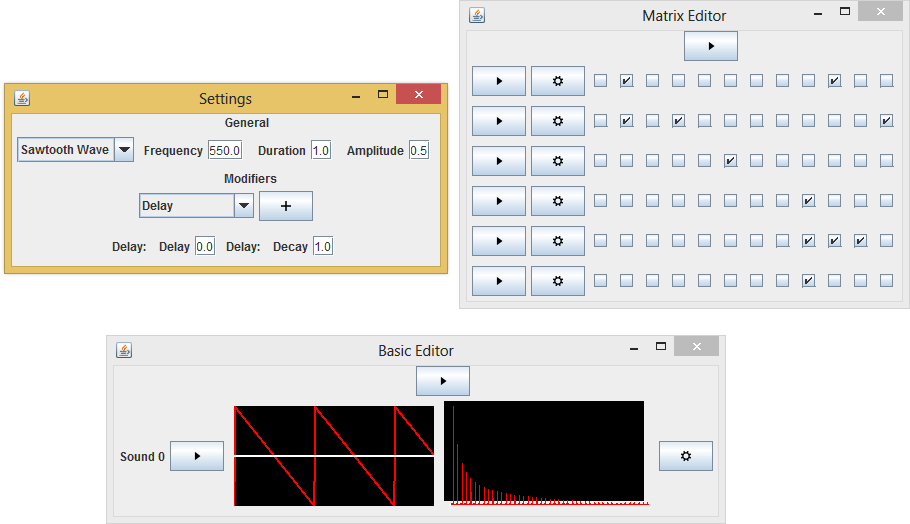
\includegraphics[scale=0.4]{global_view.png}

\section{Framework}

\subsection{Modularity}
The core of the framework is the class Sound. Everything depends on it, but we tried to limit the connections between the different parts of the framework, because we think it is generally a good practice. The model then is constructed in modules, that anyone can easily extends to its own needs. The second essential part of this design is the Player, whose implementation was inspired by the StdAudio library\footnote{http://introcs.cs.princeton.edu/java/stdlib/StdAudio.java.html}, created in Princeton, and that we limited to software generated waves but expanded with the possibility of mixing them.

Considering that we had to give the possiblity to derive both simple and more complex implementations from this framework, it was essential to keep the modules well separated.
As a result, we came up with a design where the only mandatory components to get a working application are a Sound object, a Generator and a Player.
It means that our framework could also be used as an external library, dedicated to the generation and playing of sounds.
Indeed, the data model relies on a simple array of samples, which could very well be integrated in any application requiring sound synthesis.
The generators and views by themselves could also be used as a third party library and integrated in other sound models.

\subsection{Extensibility}
When we started to think about the implementation, we wanted to give the user the ability to easily append new classes to any part of the framework.
The modularity is a first step toward this goal, the genericity of the superclasses and interfaces is the next one.
We tried not to put boundaries around the possible use cases and used our growing knowledge about object oriented programming and design patterns in this way.

\paragraph{Model View Controller}
We used extensively the Model View Controller architecture, obviously between the sound object and its views, but also between each part of the model and their associated editor.
It is applied at each level, down to the Parameter class which communicates directly with its associated Editor, allowing for it to be used in different situations, as a Modifier parameter but also as a Sound parameter.
To implement this pattern, we relied heavily on the Observer interface and Observable abstract class, part of the standard Java library.

This implementation makes it possible for a Parameter object to be updated through standard method call by its associated ParameterEditor.
He will then be able to parse the value coming from the user interface, then send back the correct value to the editor as well as notifying its Modifier that a change in the parameter's value occured.
It also means that the value of the parameter could be set from anywhere else in the class, through its standard library, but the model and the associated editor would in any case be notified of the changes.

\paragraph{Strategy Pattern}
The extensibility comes also from the use of the Strategy Pattern in the implementation both of the generators and the modifiers.
One generator must be affected to the Sound in order for it to produce a signal to be played.
The abstract class is generic, the user only needs to implement its own generate method as well as overloading the toString method (because of the user interface).

For the modifiers, they can be appended to the Sound at any moment, leading to a regeneration of the audio signal, as it happens when any parameter's value is changed.
The only extra thing needed there is an overloading of the method getParameters, which is useful for the automation of the user interface generation.
As for now no other solution has been found to this problem, although we do not think it is a big issue, it is important to note.

\subsection{Flexibility}
An objective was to come up with a structure allowing the user to build upon it both command line utilities or graphical interfaces.
As the requirements were to provide a graphical user interface, we decided to design a flexible one.
It means that a client application could very well be working fully from the command line, though we didn't provide any example of this kind, because it wasn't our goal.
It could also be an hybrid, like the basic editor, which is taking its initial input from the console and then provides a graphical interface for further tweaking, playing and visualization of the signals.
Finally it can be fully graphical, as you can see in the matrix editor implementation, which provides a prebuild set of sounds, and the panels to adjusts their parameters further on.
\section{Views}	
We think having the opportunity to display the model through different perspectives gives another dimension to the framework. This is why having a visual representation of the sounds was also one of our objectives. To fit to the concept of extensibility, we wanted the class user to be able to add more views, which is done just by implementing the View interface and create a new one. The spectral view relies on the use of an external ressource, the FFT\footnote{http://nayuki.eigenstate.org/page/free-small-fft-in-multiple-languages/ by Nayuki Minase/} class. The reason why we choose this resource is because it is more flexible than most of the transform algorithms we can find on the web, which usually require an array that is a power of 2 as parameter. Indeed, the size of the sound data array depends on the duration the user has select therefore we needed a more flexible approach. The one we chose, checks the size of its given parameter and execute the right algorithm either the Cooley-Tukey decimation-in-time radix-2 algorithm if the size of the given array is a power of 2 or the Bluestein's chirp z-transform algorithm.

\section{Basic Editor}

The basic editor is a really simple application whose purpose is only to demonstrate, in parallel with the Matrix editor, different use cases of the framework.

It takes the input from the command line, in the form of a frequency, a duration and an amplitude, repeted any number of time.
The user input is then processed by a test class, which instanciate a player object, fills it with newly created sounds, and then pass it to a basic editor object.
It is done this way because it keeps each part of the application separated.
The player object could very well be used by calling its methods and without any need of an editor.
The views as well could be appended to the sounds and rendered on a JFrame.

The user can then do further modifications on the different sounds, visualizing the modifications both on a temporal view and a spectral view.
The SoundEditor associated to each sound can be opened easily, and new modifiers can be appended.
Because it relies on a player object, it can mix the different sounds or play them separately.

\section{Matrix Editor}

The inspiration for the non-trivial application came from an embedded ActionScript application\footnote{http://www.hisschemoller.com/2009/step-sequencer-drum-machine/} allowing an easy creation of sound patterns.

It basically relies again on a dummy class, which provides the Player object to the editor.
However this time all the sounds instanciations are done internally, to display right from the beginning a pre-filled matrix of sounds.

Of course the user can tweak each of them like in the basic implementation, but this time he can also creates sound patterns by choosing which sound to play when.
Unfortunately we didn't had the time to pursue farther on this application, and one major issue was raised during the implementation.

To pursue in this way it would be necessary to use different threads, one to handle the graphical part of the application, the other one dedicated to the audio playback.
We would have liked to dig deeper in this field, because we worked with threads in previous C++ courses and were interested in their implementation in Java.

Without multithreading, it is difficult to implement totally what we imagined at the beginning for the matrix editor, because the interface simply freezes during the playback and thus can't handle user inputs and loop on the pattern.
The idea behind this editor being reactivity and freedom in the creation, we're facing a wall here with a simple thread.

To fit the original idea it would also be necessary to add sleeping timers inside the playing loop in order to give each column a definite duration, independent of whether there is a sound playing on this column or not.
For the moment these empty columns are simply skipped, thus not allowing real liberty in the creation of the patterns.

The last issue concerns the playing methods.
Indeed, it actually does not allow to start sounds "on top" of an already playing one.
If we take a look at the ActionScript implementation, we realize that each sound is played entirely, and the sounds starting later on is mixed with it, in real time.
The actual construction of the player object does not allow this type of operation.
Although we tried a refactoring of the code, we decided to put it aside and focus on other issues, because without multithreading does functionalities do not make real sense.

\chapter{Testing}

Testing was by far the most difficult part of the project.
Being really new to this somewhat delicate topic led us to real problems in the definition of the testing procedures.

Firstly, we didn't really know what in this kind of application should have been tested thorougly, and this also comes from the fact that the separation in multiple sub modules makes it difficult to test whole features.

Then, when we found the critical spots, implementing tests in scalacheck seemed very difficult, because we lack knowledge in this language and way of thinking.

Finally we tried to rely on preconditions and postconditions, checked with assert statements in the places we thought were at risk.

We know that the learning curve can be quite steep before gathering enough knowledge and actually writing good unit tests, but we will definitely have a closer look to those subjects in the future, because it is essential.

\chapter{Some code we are proud of}

\section{Prototypers}
One thing we are rather satisfied with is the solution we found for the tricky problem of listing the possible generators and modifiers for the user to choose.
The core of the problem was again to offer flexibility and extensibility, so we needed to find an easy way for the user to add its own custom classes to the selectors.

The solution has been found by merging the ideas from two famous design patterns, the Factory Pattern and the Prototype Pattern.
We created prototypers class which have static methods to fill an array with prototypes and then return this array when needed, to fill the JComboBox.
The prototypers are filled by methods of the Editor abstract class, which inserts the basic modifiers and generators we provide with the framework.

Adding custom ones is then simply done in the inheriting class of Editor (here BasicEditor and MatrixEditor) by overloading the methods, and then either filling only with new prototypes or combining them if the superclass method is called.

\section{Karplus-Strong algorithm}
The most pleasant implementation has definitely been the Karplus-Strong string synthesis algorithm.
Suggested in the project description, we decided to implement it in order to provide something different from the classic wave generators.

Our code is based on an exercise by Timothy Wood\footnote{http://faculty.cs.gwu.edu/~timwood/wiki/doku.php/teaching:f2012:cs2113:ex5} from the George Washington University.
The result is really great, and we would have liked to have the time to implement other generators of this kind.
They make our framework really look like a small toolkit for sound creation, and they are really fun and rewarding to implement.

\chapter{Results}

To conclude we want to say that we have been really interested in this project, because the applications are real, so the inspiration came easily.
We had never used Java previously, however we did some C++ in previous courses or as a personnal interest.
The Java way of making Object Oriented Programming seemed quite easy to catch, and we found that our efficiency over this few weeks wouldn't have been so great in C++.

Obviously the job is not done, and maybe we will continue to build upon this framework in the future.
It lacks a lot of cool modifiers, and some features which are actually made possible in the code (muting sounds in the Player) were not implemented because it wasn't on the top of the priorities.
We also wanted to implement the possiblity to play external sounds, from files, and also having saving methods.
It wasn't done because of a lack of time, but we think it can be added easily, directly in the Player for the first point, and through a Recorder class for the second.

The most frustrating aspect is probably the impossibility to properly implement the matrix editor because of this mutlithreading issue that should have come earlier to our minds but simply didn't.

Finally we would like to thank our supervisor and teacher, Dr. Veronica Gaspes. She supported us totally, gave us the hints we needed to solve the big issues, incited us to go further and at the same time complimented us about what was actually working.

\end{document}